Compute the first difference of the log-transformed of the original series. Examine its sample \textbf{acf} plot and compare it with the \textbf{acf} plot of the residuals in part (c). Make sure to display your plots.

\nl Using the following code:
\begin{verbatim}
    diffAirpass <- diff(stableAirpass)
    acf(diffAirpass)
\end{verbatim}

\notab{\center{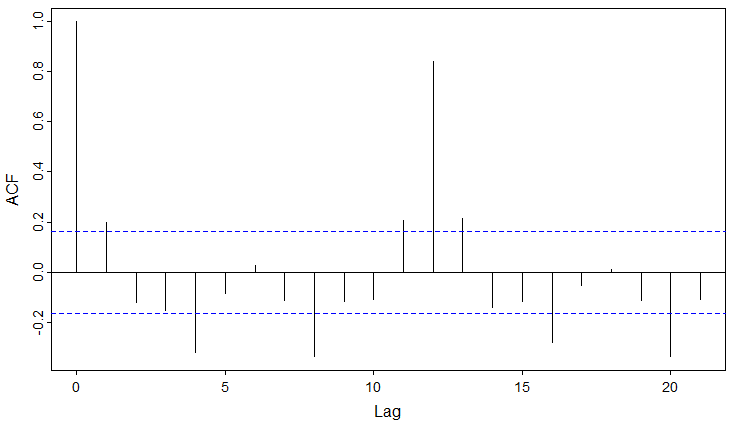
\includegraphics[width=4.5in]{img/7d.PNG}}}

\nl The ACF of the first difference has less data points spiking above the blue dashed line than the linear regression did. This indicates that the residuals of the first difference are less correlated. The first difference stabilizes near zero much faster than the linear regression model, of which slowly decreases in residual size over time. Both graphs still follow a cyclic pattern of period 12.